\chapter{Resultados}
%\section{Resultados en Simulaci\'on}
\section {Resultados del Controlador Polar}
\begin{figure}%[ht!]
  \centering \footnotesize
  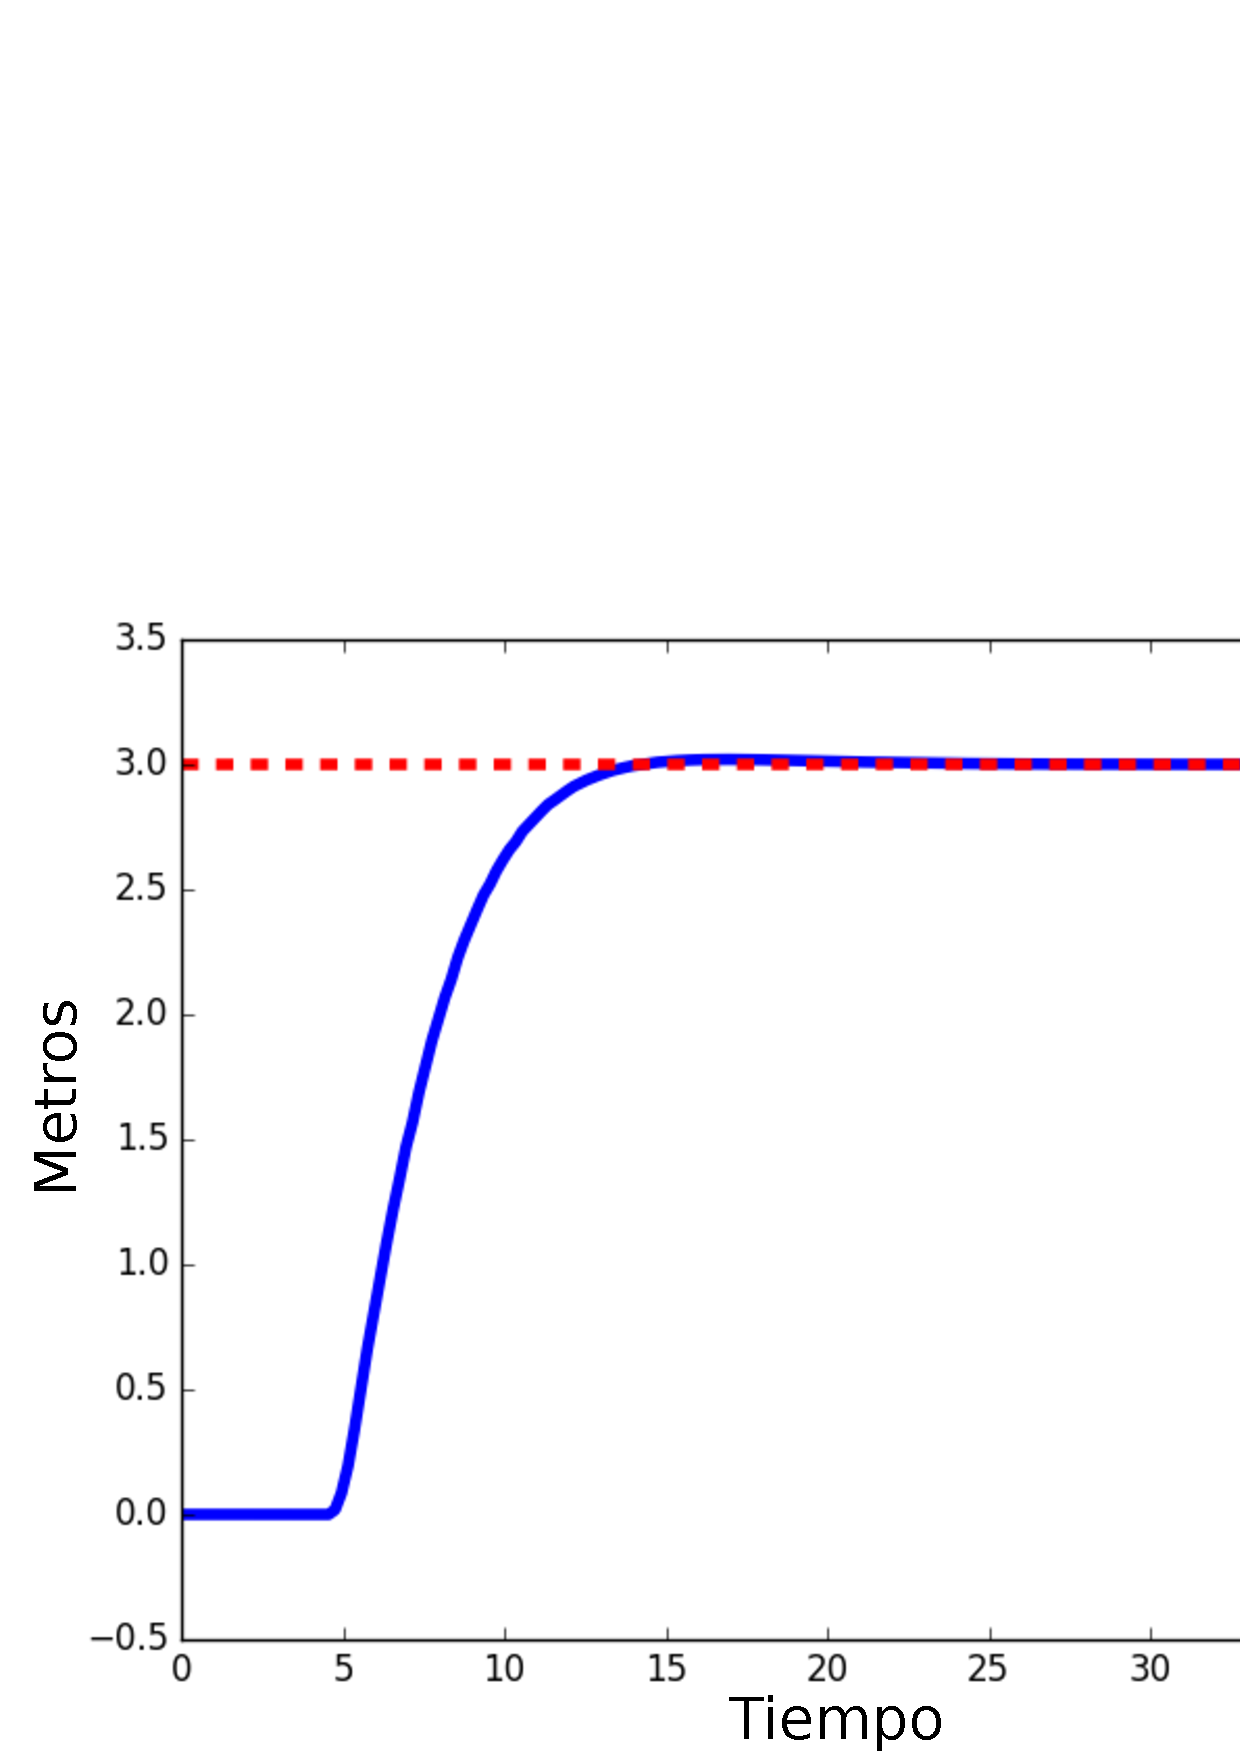
\includegraphics[width=0.40\textwidth]{images/tvsxy_tesis.png}
  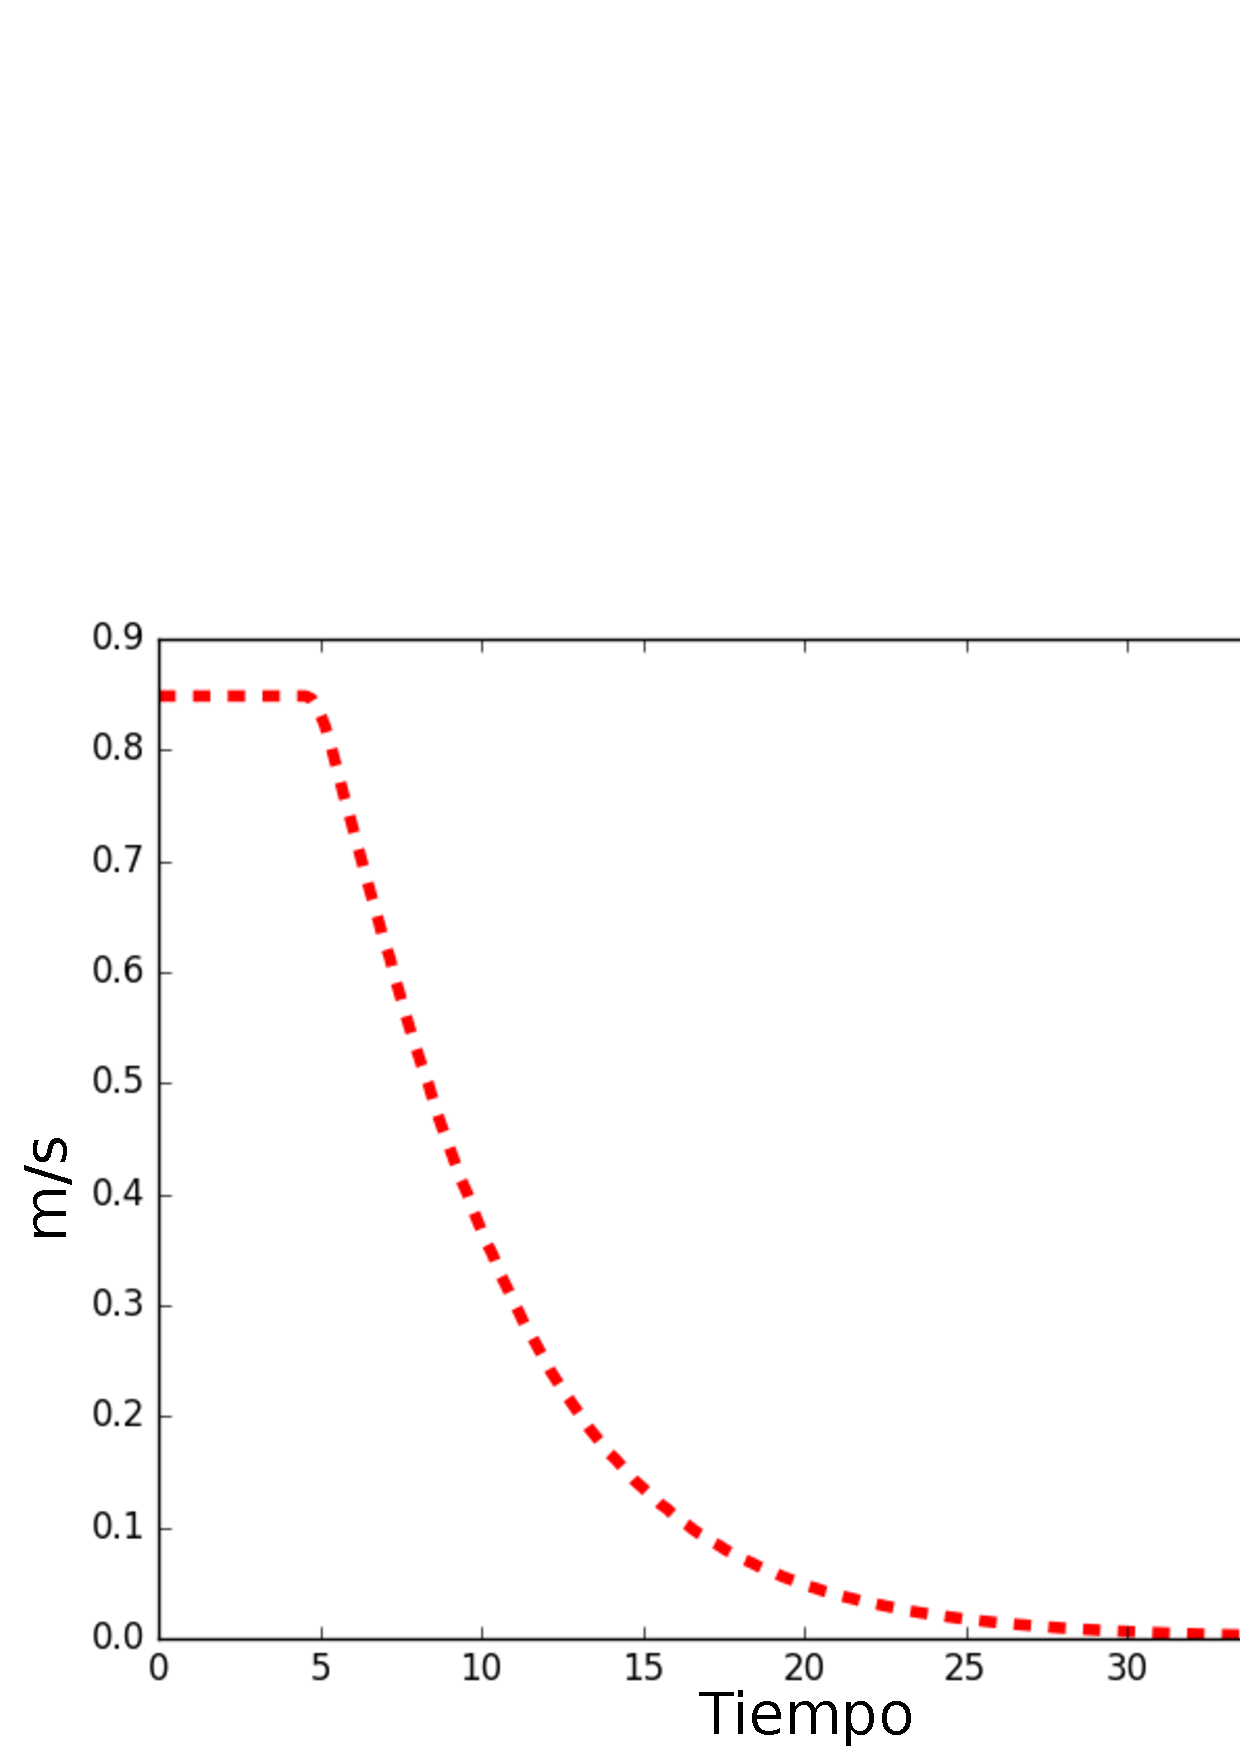
\includegraphics[width=0.40\textwidth]{images/tvsv_tesis.png}
  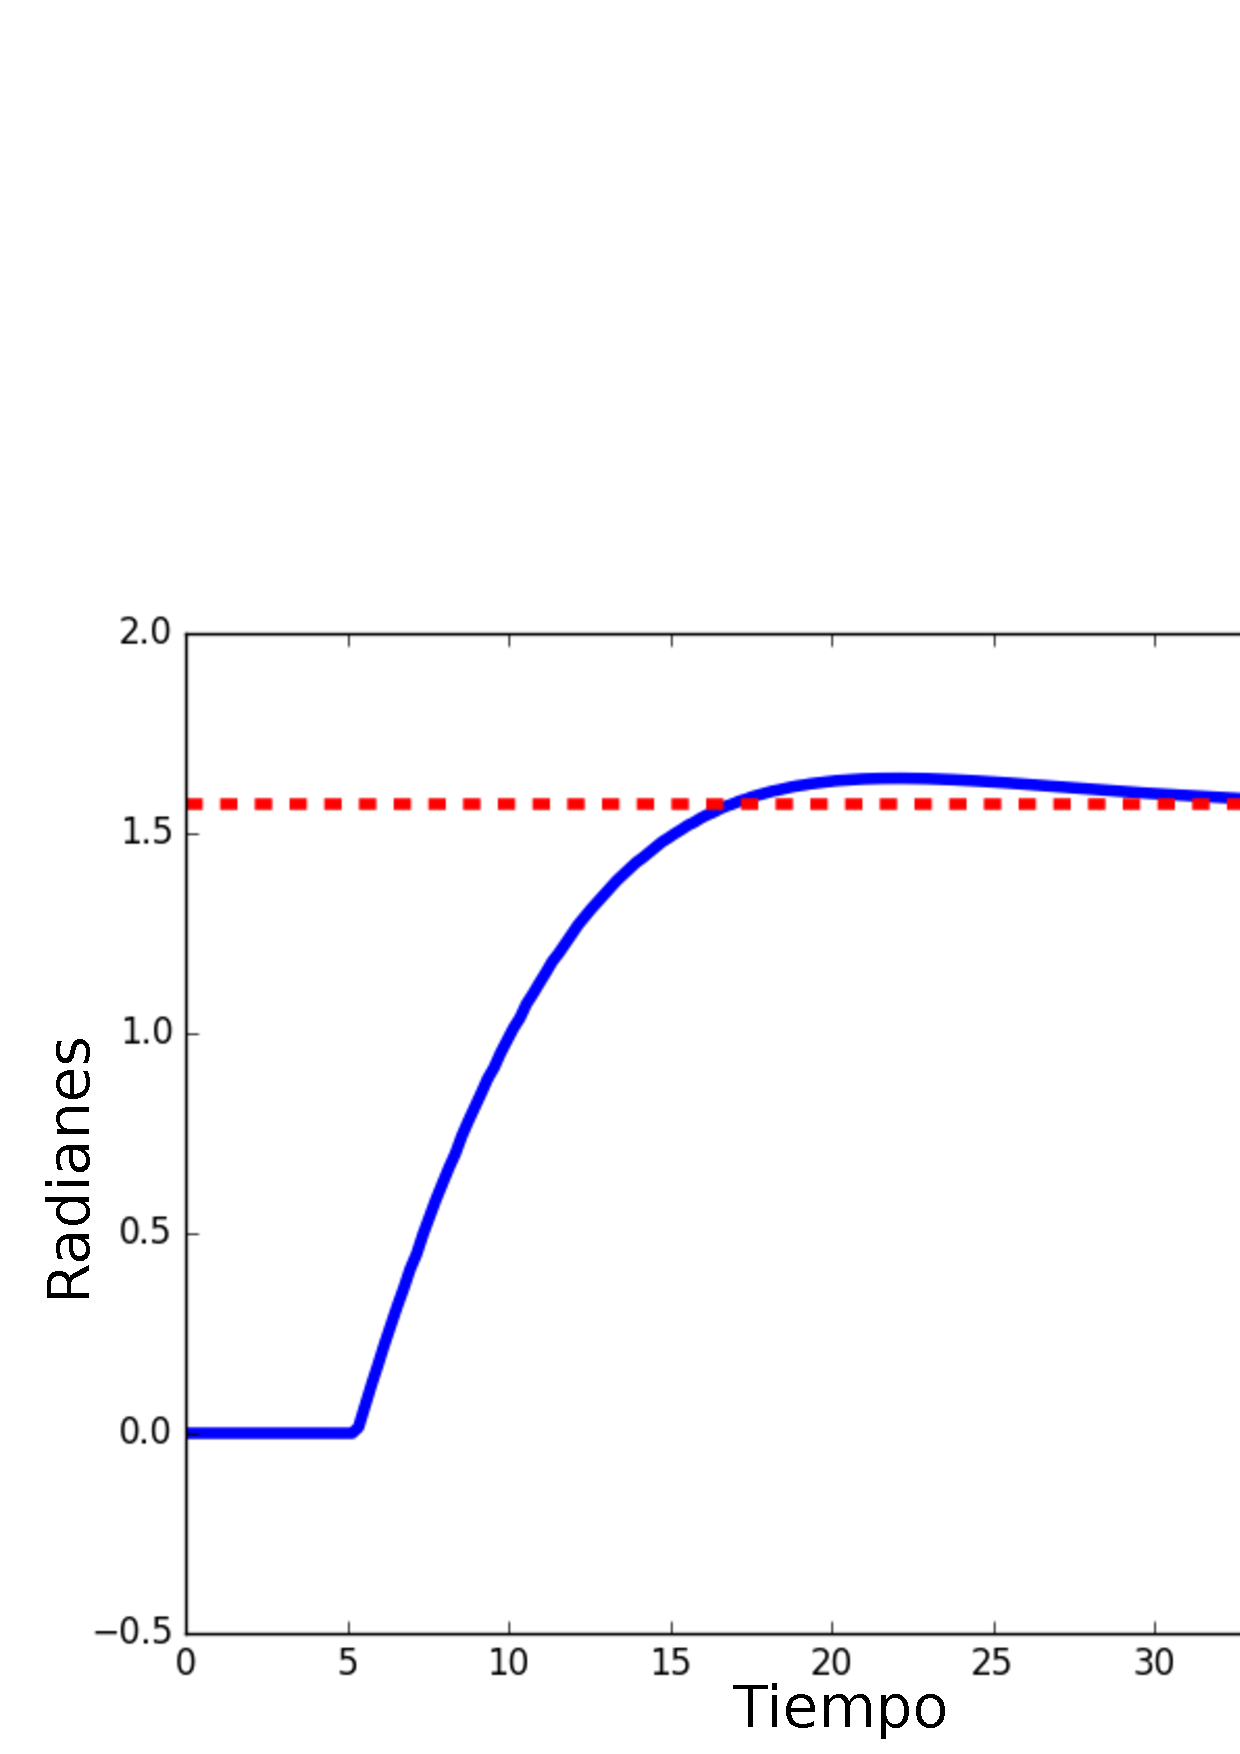
\includegraphics[width=0.40\textwidth]{images/tvstheta_tesis.png}
  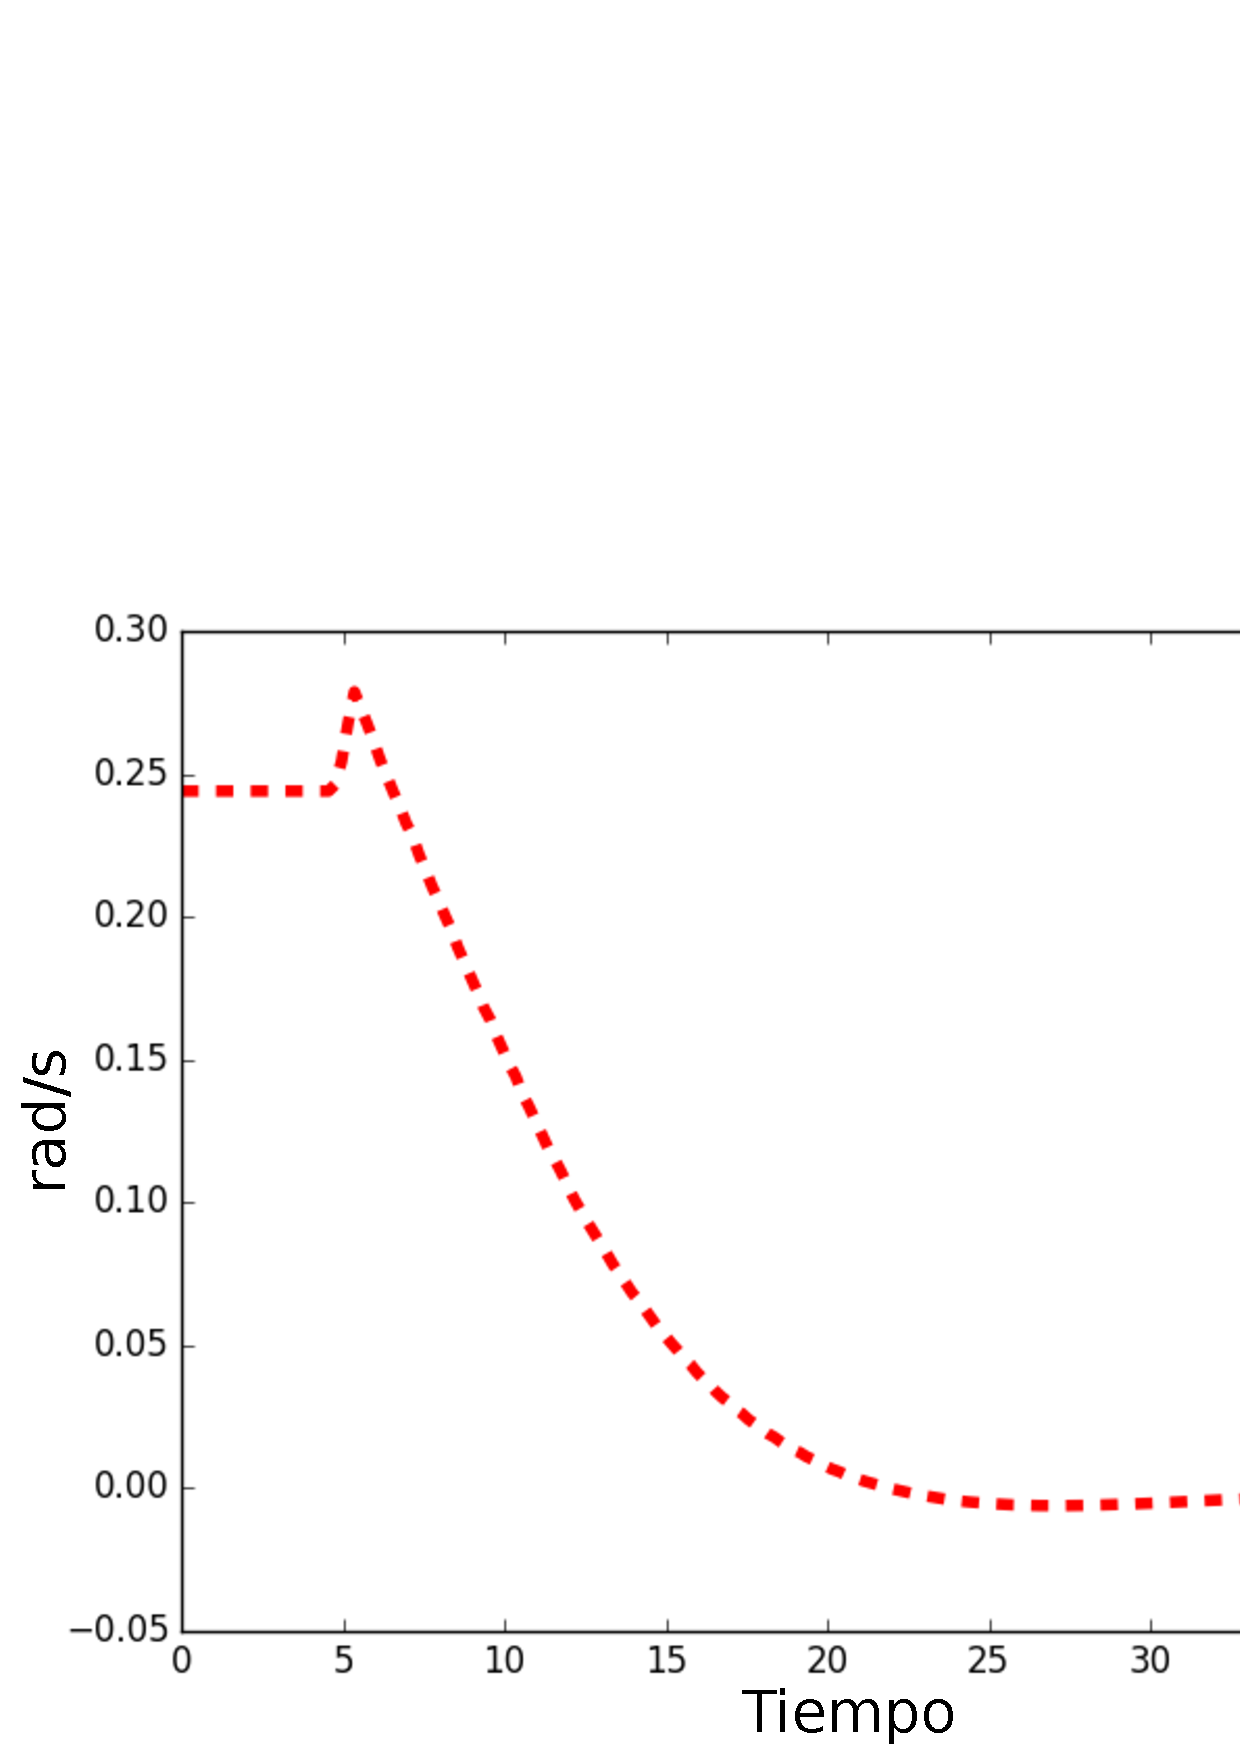
\includegraphics[width=0.40\textwidth]{images/tvsomega_tesis.png}
  \captionsetup{font=footnotesize}
  \caption{Evolución temporal de las variables de estado usando el controlador polar 
  para lograr una posición deseada dada por $x = 3, y = 3, \theta = 90$}
  \label{f:PolarControl}
\end{figure}
Para probar el controlador polar, se usó una simulación dinámica en Gazebo con el robot 
Kobuki sin obstáculos, y las variables de estado que incluyen velocidad, posición y 
orientación se obtuvieron en línea a partir de la odometría simulada. Usando la información 
de esta odometría, el controlador se aplicó en línea. Para estas pruebas, la posición del 
objetivo era $(x = 3, y = 3)$ y la orientación del objetivo $\theta = 90^{\circ}$. La 
figura \ref{f:PolarControl} (a) muestra la evolución temporal de la posición ($x$) donde 
se logra una convergencia a la posición deseada en menos de 20 segundos. Esto se debe a 
la distancia hacia el obstáculo. Diferentes distancias conducen a diferentes tiempos de 
convergencia, y la tasa de convergencia también se puede modificar cambiando las 
ganancias en \ref{eqn:w} para la velocidad angular, y en \ref{eqn:v} para la velocidad 
lineal. Las otras subfiguras en la figura \ref{f:PolarControl} muestran la evolución 
temporal de la velocidad lineal en $x$, la orientación y la velocidad angular. Para la 
orientación, hay un sobreimpulso que se debe a la excesiva dependencia del controlador 
en la posición en lugar de la orientación.
%\section{An\'alisis del mapa obtenido}
%\section{Resultados en un ambiente real}
\section{Resultados del Sistema de Navegación}
\begin{figure}%[ht!]
  \centering \footnotesize
  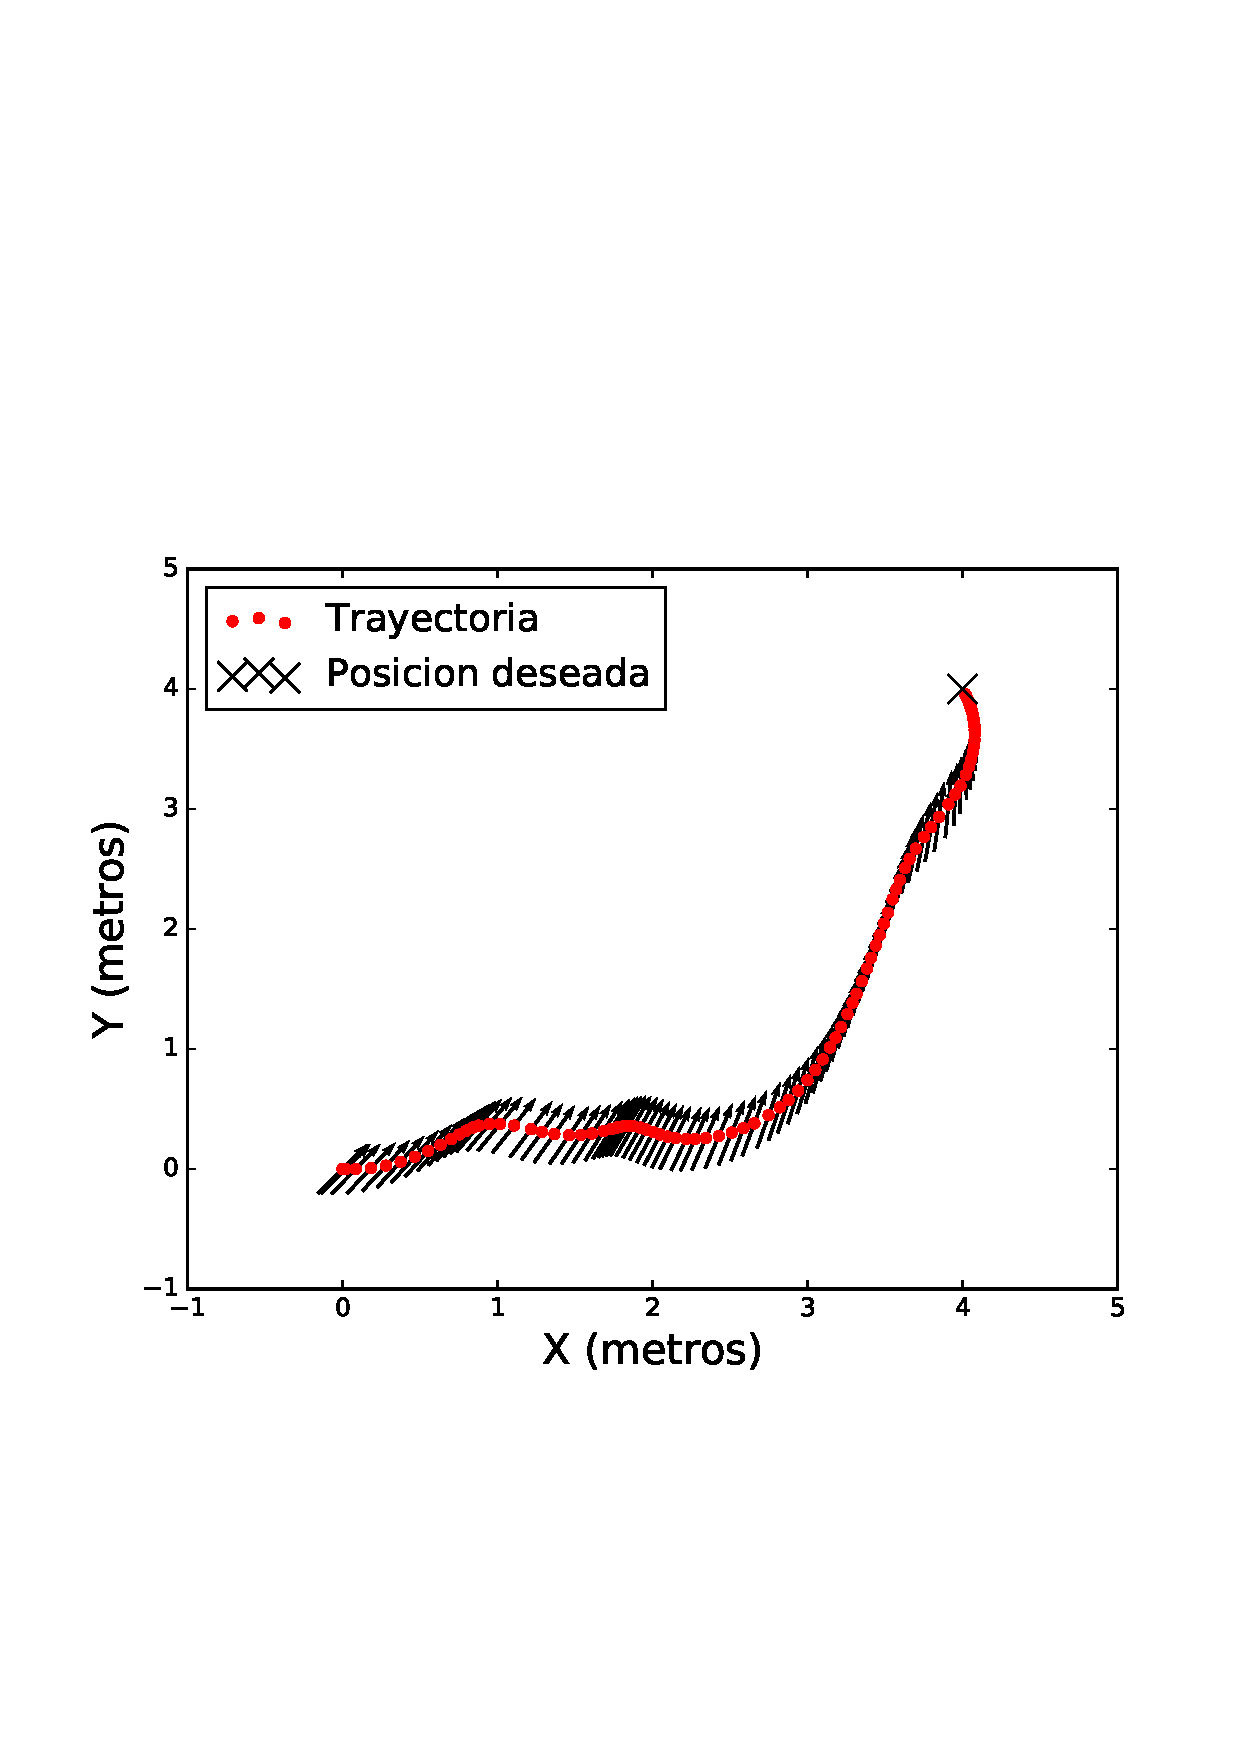
\includegraphics[width=0.40\textwidth]{images/attr_kbki.png}
  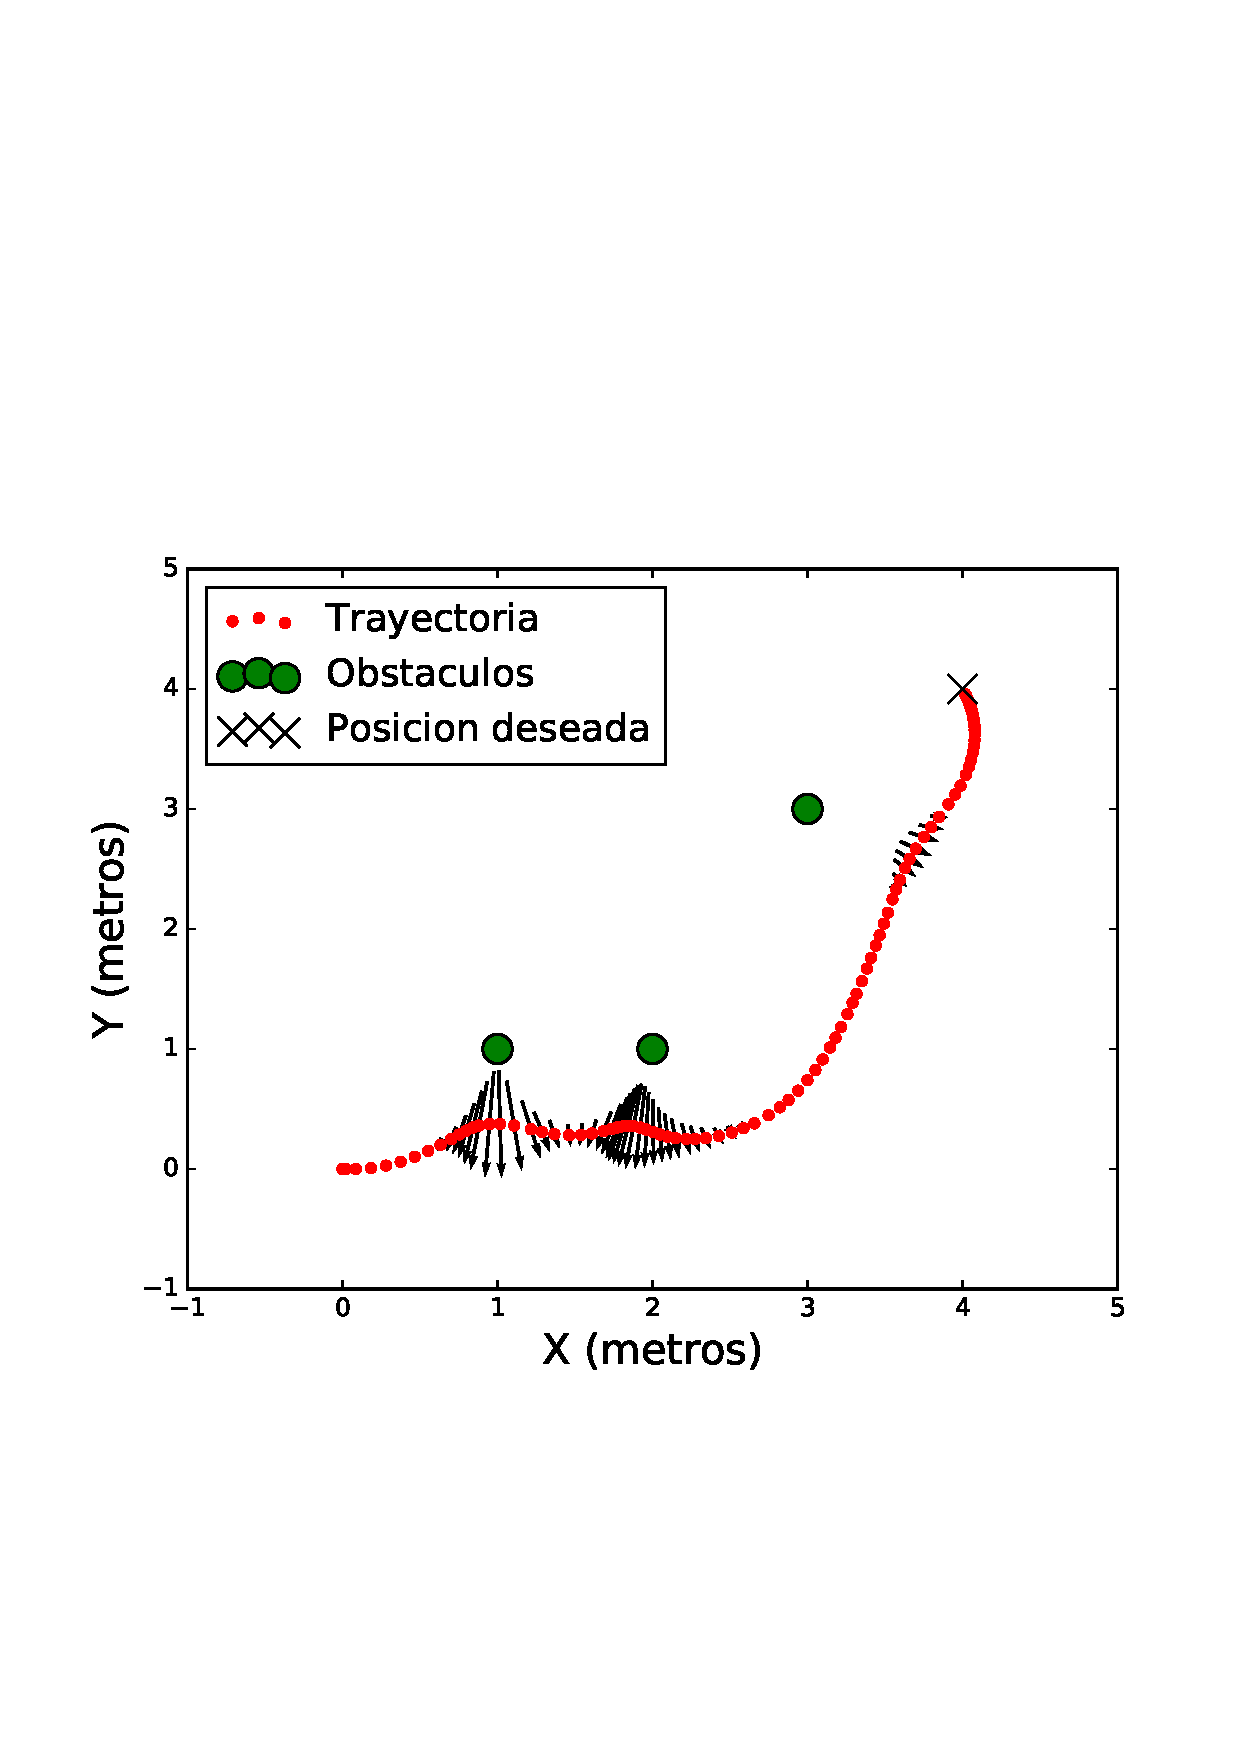
\includegraphics[width=0.40\textwidth]{images/rep_kbki.png}
  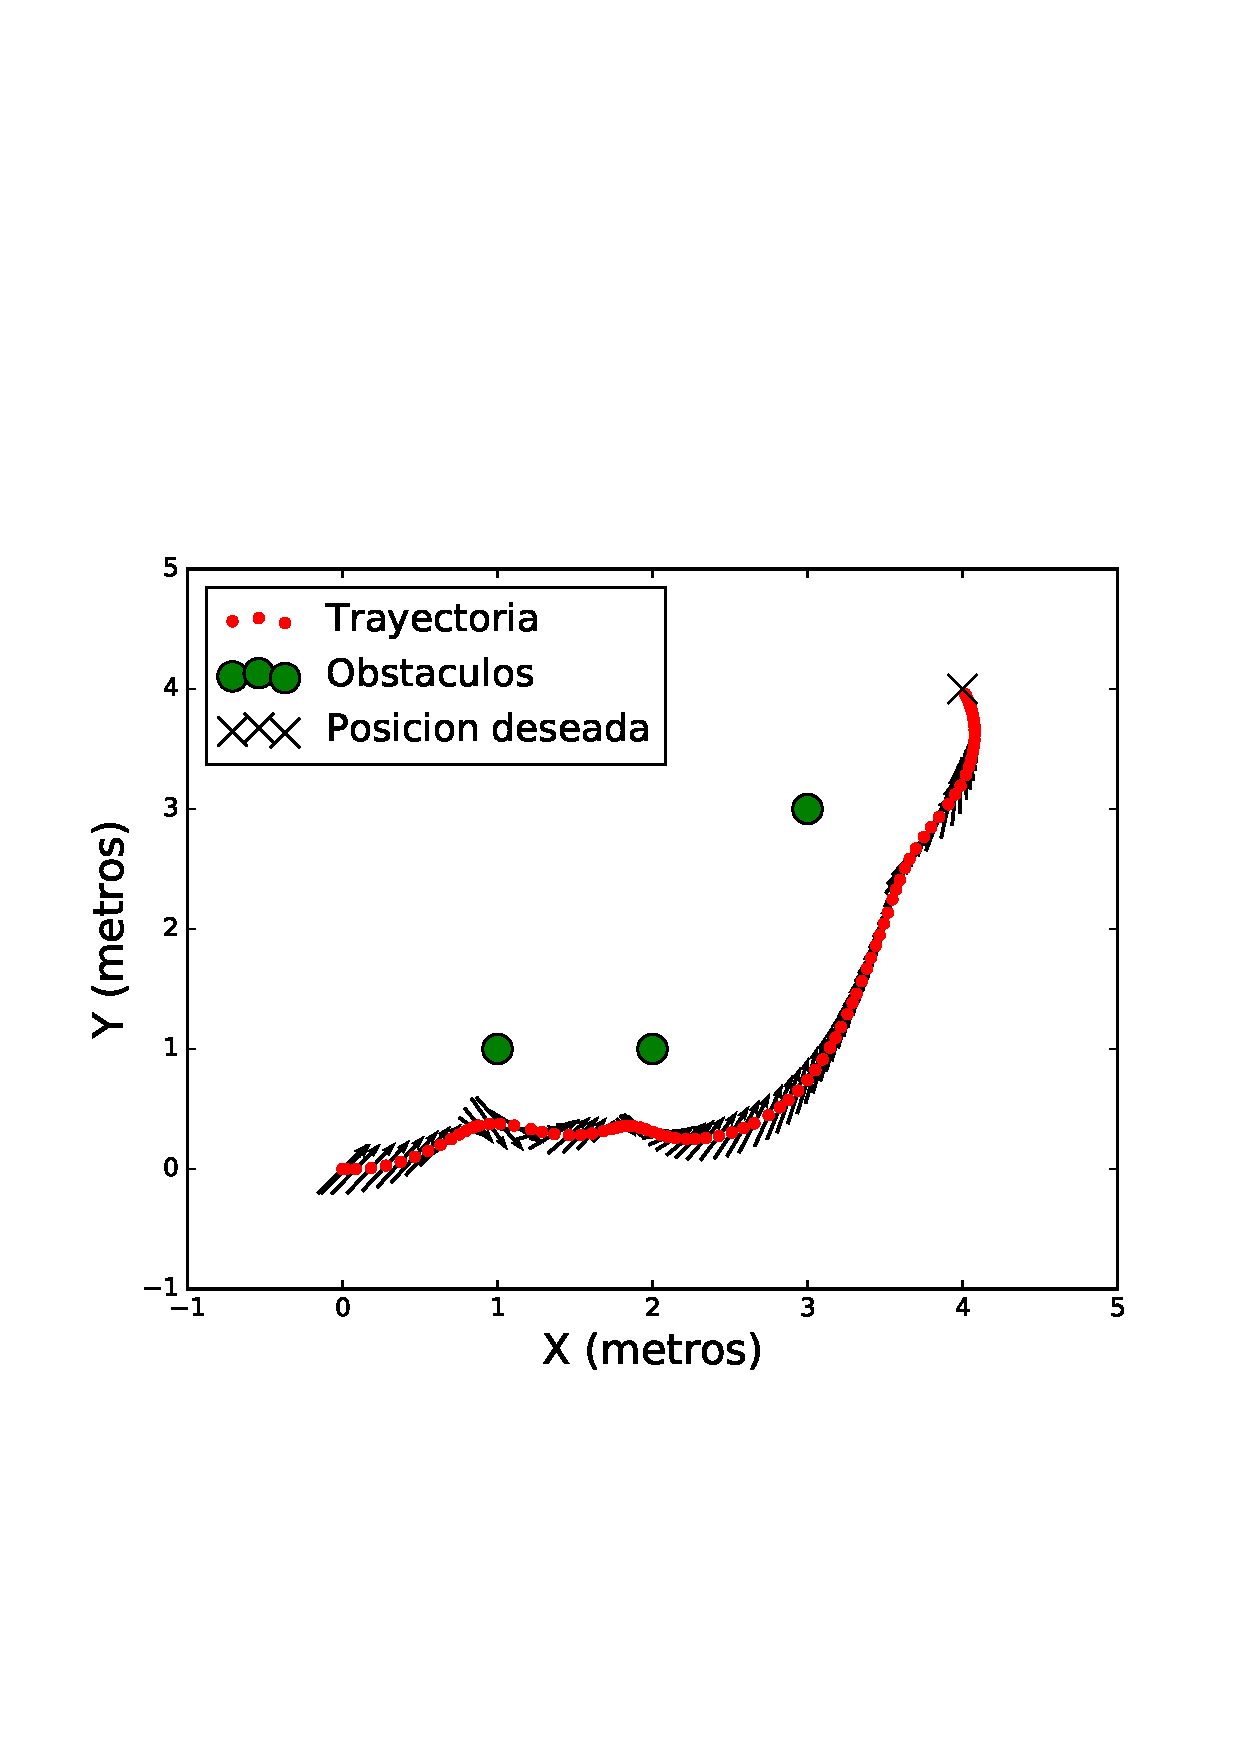
\includegraphics[width=0.60\textwidth]{images/nav_kbki.png}
  \captionsetup{font=footnotesize}
  \caption{Navegación autónoma implementada en el robot diferencial Kobuki.}
  \label{f:kbki_APF}
\end{figure}
La metodología propuesta se implementó como un algoritmo iterativo en el robot Kobuki. 
Como se se describe en la sección \ref{sec:autonomia}, el algoritmo toma iterativamente 
posiciones medias de objetivos a través del campo potencial artificial y el controlador 
polar impulsa al robot a través de ellas. Expusimos al robot a diferentes obstáculos cuyas 
posiciones fueron conocidas a priori. La figura \ref{f:kbki_APF} (a) muestra las fuerzas de 
atracción para cada posición (puntos rojos) en las que el algoritmo se itera en el entorno 
bidimensional dentro del movimiento del robot. Para cada posición, el campo de potencial 
atractivo que se verifica con las flechas. La figura \ref{f:kbki_APF} (b) se compone de las 
fuerzas de repulsión basadas en los obstáculos, que se muestran como marcadores verdes. Para 
cada obstáculo, la magnitud de las fuerzas aumenta cuando el robot está más cerca y su dirección 
señala los obstáculos, permitiendo que el robot los evite. La figura \ref{f:kbki_APF} (c) muestra 
la superposición de ambas fuerzas con los obstáculos reales. Cada fuerza proporciona una posición 
de meta intermedia para el robot, que constituye la posición deseada continuamente actualizada 
para el controlador polar. Aunque las fuerzas cercanas a los obstáculos tienen un alto índice 
de cambio, la trayectoria es suave. Esto demuestra la efectividad del controlador polar a pesar 
de las características no holonómicas del robot.

\section{Resultados de la Navegación Autónoma con el Lidar (2D)}
\begin{figure}%[ht!]
  \centering \footnotesize
  \includegraphics[width=0.40\textwidth]{images/kobuki_201.jpg}
  \includegraphics[width=0.42\textwidth]{images/fattr_lidar.png}
  \includegraphics[width=0.42\textwidth]{images/frep_lidar.png}
  \includegraphics[width=0.42\textwidth]{images/fnav_lidar.png}
  \captionsetup{font=footnotesize}
  \caption{Campos atractivos y repulsivos, y la trayectoria que el robot real sigue 
  usando datos en línea provenientes del sensor lidar montado en la parte superior.}
  \label{f:kbki_autonomo}
\end{figure}
Para probar la autonomía del robot móvil en un entorno real, se usa un lidar (RPLidar A2) 
que se instaló encima del robot Kobuki. El uso es la actualización continua de las posiciones 
de los obstáculos a medida que el robot se mueve. El robot usa tópicos creados en ROS para 
obtener la información del sensor que se compone del rango y la orientación de cada punto 
medido, a medida que el lidar gira. La información de rumbo y alcance se convirtió a coordenadas 
cartesianas para conocer las posiciones cartesianas de los obstáculos dentro del espacio de 
trabajo, que es la entrada al algoritmo principal. Para que el kobuki pueda moverse dentro 
del mapa generado por el lidar, el marco de referencia del robot se tomó como el marco del 
lidar. Entonces, el algoritmo de navegación autónomo podría usar estas coordenadas del 
obstáculo para generar su propia trayectoria evitando obstáculos. Para toda la prueba, se 
colocaron dos cajas en el espacio de trabajo, como se ve en la figura \ref{f:kbki_autonomo} 
(a). La posición del objetivo era ($x = 4, y = 0$). La figura \ref{f:kbki_autonomo} (b) muestra 
la trayectoria del robot en azul y las flechas que indican la fuerza que lleva al robot a la 
posición deseada. La figura \ref{f:kbki_autonomo} (c) muestra el mapa completo, donde los puntos 
verdes representan el entorno, detectados por el lidar, donde se mueve el robot. Como se 
observa, estas flechas apuntan hacia afuera del obstáculo, proporcionando autonomía al robot 
mientras intenta alcanzar la meta. Finalmente en la figura \ref{f:kbki_autonomo} (d) se muestra 
toda la fuerza de navegación que impulsa el movimiento.


  

